
\section*{Facilities, Equipment, and Other Resources}

PI Pandey's research group uses high-performance computing infrastructure at the University of Utah. PI Pandey is also an affiliate with Lawrence Berkeley National Lab his research group also uses NERSC computing facilities at Lawrence Berkeley National lab.

\subsection*{University of Utah}
The University of Utah provides several computing facilities for instructional and research use. The campus network backbone is a 40+Gbps network with a 100 Gbps research DMZ\@. The campus attaches via redundant 10 Gbps links to the Utah Education Network (UEN) which provides commodity internet and research connectivity. UEN maintains multiple gigabits of commodity from various carriers at strategic points throughout the state. For research connectivity, UEN connects via 10 Gbps directly with the 100 Gbps backbone of Internet2, both at the Salt Lake Level3 PoP. The University of Utah’s School of Computing attaches via redundant 10 Gbps connections to the campus backbone routed via OSPF\@; this provides desktop connections with 1 Gbps ethernet.

\subsubsection*{School of Computing}
The School of Computing’s computing infrastructure supplies many centralized services, including shared disk space (100 Terabytes), time, web/cgi/php, s/ftp, firewall, backups, printing resources, authentication (AD/LDAP/NIS), vpn, ssh/interactive servers, door lock access, and email. The core of the server infrastructure runs on VMware’s Enterprise virtualization products. Most services run on VM-Linux-based hosts, with some additional services being served from Windows machines. The School of Computing’s core instructional computing facility is the Computer Aided Design and Engineering (CADE) Lab. The CADE Lab includes approximately 75 personal computers running Centos 7.2 Linux with the 3.10 kernel, deployed on hardware equipped with an 3.60GHz Intel Core i7-4790 Processor, 32~GB DDR3 1600~MHz overclocked RAM, GeForce GTX 770/970 with 4~GB of memory, and a 240~GB Intel 540 Solid State Drive.

\subsubsection*{Center for High Performance Computing}
The University of Utah’s core research computing facility is the Center for High Performance Computing (CHPC), which supports the deployment and operation of large-scale and high performance computational resources, while also facilitating use of these resources through advanced user support and training. The CHPC also serves as an expert team to broadly support the diverse research computing needs on campus, in- cluding support for big data, big data movement, data analytics, security, virtual machines, Windows science application servers, protected environments for data mining and analysis of protected health information, and advanced networking. The CHPC manages over 22,000 cores and over 13 PB of RAID configured spinning disks. CHPC also leverages the national cyberinfrastructure for resources and training, including serving as partners in the ACI-REF (Advanced Cyberinfrastructure Research and Education Facilitators) program and as a member of RMACC (Rocky Mountain Advanced Computing Consortium).


\subsection*{Lawrence Berkeley National Laboratory}
%%%%%%%%%%%%%%%%%%%%%%%%%%%%%%%%%%%%%%%%%

Lawrence Berkeley National Laboratory (Berkeley Lab) is the leading provider of computing and networking resources supporting the DOE Office of Science's research mission. Berkeley Lab researchers have access to leading-edge computing platforms and services at the National Energy Research Scientific Computing Center (NERSC) and have 100 Gbps connectivity to other national labs and institutions via ESnet, DOE's Energy Sciences Network, both of which are managed by Berkeley Lab. The Lab also manages several departmental clusters.

\subsubsection*{NERSC}

NERSC is the mission high-performance computing facility for the DOE's Office of Science, supporting large-scale simulations and a growing workload in data analysis from the DOE's experimental and observational facilities. Managed by DOE's SC Advanced Scientific Computing Research program and operated by Berkeley Lab, in 2021 NERSC served more than 8,000 scientists, working on about 900 research projects, with users from all 50 states and Washington D.C. that span the range of SC scientific disciplines. NERSC has a significant impact on scientific research; e.g., proposals for 2020 allocations cited over 2,000 distinct refereed publications that used NERSC\@. In 2020, 61\% of NERSC users came from universities, 30\% from DOE national laboratories, and the remainder from other government laboratories, industry, and nonprofits.

\begin{figure}[ht]
 \begin{center}
    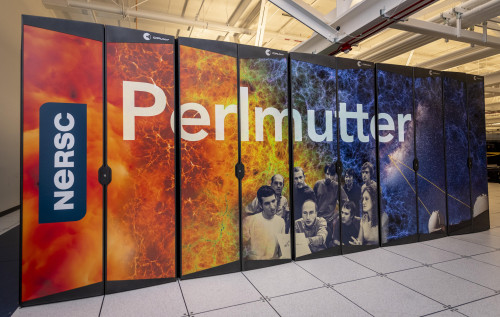
\includegraphics[width=0.5\textwidth]
    {images/perlmutter.jpg}
 \end{center}
\end{figure}

In addition to providing world-class supercomputers, NERSC offers expert support to ensure that its users make the most efficient and effective use of the facility's resources. NERSC staff help users optimize their applications for advanced computing architectures, and they engage with users from experimental facilities to run complex workflows on NERSC systems. Increasingly, NERSC staff aid users in implementing advanced analytics and machine learning capabilities into their applications and workflows.

In 2021 NERSC unveiled its newest flagship supercomputer, Perlmutter, a Cray Shasta system based on NVIDIA A100 GPUs with new tensor core technology, AMD EPYC CPUs, and the HPE Cray ``Slingshot'' high-speed interconnect. The system is named in honor of Saul Perlmutter, an astrophysicist at Berkeley Lab and a professor of physics at UC Berkeley who shared the 2011 Nobel Prize in Physics for his contributions to research showing that the expansion of the universe is accelerating. Perlmutter is ranked as the 5th most powerful supercomputer in the world as of November 2021 and includes several innovations designed to meet the diverse computational and data analysis needs of NERSC's user base and speed their scientific productivity, including  an all-flash scratch filesystem. Developed by Cray to accelerate I/O, the 30-petabyte Lustre filesystem will move data at a rate of more than 4 terabytes/sec.

\begin{figure}[ht]
 \begin{center}
    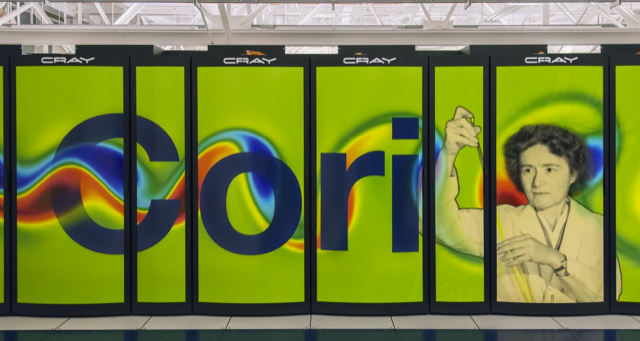
\includegraphics[width=0.6\textwidth]
    {images/cori.png}
 \end{center}
\end{figure}

NERSC also hosts an Intel-based Cray XC40 with a peak performance of 30 petaflop/s. Named ``Cori'' in honor of biochemist Gerty Cori, the first American woman to receive a Nobel Prize in science, the system delivered over 9 billion core hours in 2020 to the DOE SC user community and has several features that benefit data-intensive science. The system includes more than 1,600 Intel Xeon ``Haswell'' compute nodes and over 9,300 nodes of the Intel Xeon Phi processors (code-named Knights Landing, or KNL for short).  Cori uses the Cray Aries interconnect, a dragonfly network topology that provides scalable bandwidth.


NERSC has several storage platforms, including the Community Filesystem, a global file system available on all NERSC computational systems. It offers users a platform for collaboration and data sharing. NERSC systems are also connected to a High Performance Storage System (HPSS) for archival storage. NERSC's HPSS system currently contains more than 200 petabytes, making it one of the world's largest unclassified archival storage systems.


\subsubsection*{ESnet}

\begin{figure}[ht]
  \begin{center}
    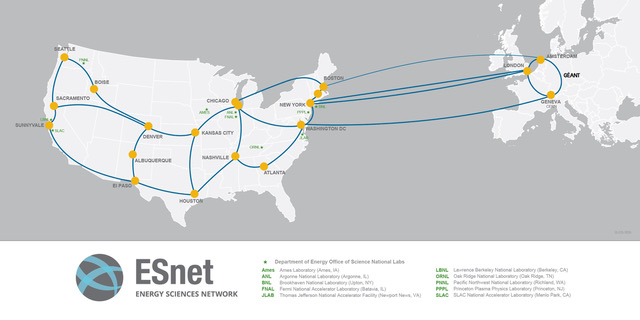
\includegraphics[width=0.95\textwidth]
    {images/esnet.jpeg}
  \end{center}
\end{figure}

ESnet interconnects the DOE's national laboratory system, dozens
of other DOE sites, and $\sim$200 research and commercial networks around
the world, enabling tens of thousands of scientists at DOE laboratories
and academic institutions across the country to transfer vast data
streams and access distributed research and computing resources in
real-time. ESnet achieves this by providing high-bandwidth, reliable
connections that enable many thousands of the nation's scientists
to collaborate on some of the world's most important scientific
challenges including energy, biosciences, materials, and the origins
of the universe. ESnet operates what is essentially the Department's
circulatory system for the movement of large-scale scientific data,
providing real-time networking to many thousands of users across
the entire DOE complex.

Access to Berkeley Lab's computational and experimental facilities
from anywhere in the U.S.~or the world is provided by ESnet. ESnet
has extended its connectivity to Europe with four 100-Gbps connections.
